\chapter[プルームモデルに従う火山ガス分布のシミュレーション]{プルームモデルに従う火山ガス分布のシミュレーション}
\label{chapt4}

本章は, これまで用いてきた区間ごとに火山ガス濃度が一定と仮定した理想モデルを発展させ,
大気中での移流および拡散を考慮したプルームモデルに基づく火山ガス分布を導入し,
より現実的な測定条件下におけるラマンDIAL観測性能について検討する.
特に, 大気の拡散条件や火口位置の違いが,
ライダー測定における距離分解能および濃度推定精度に与える影響を数値シミュレーションにより評価する.

\section{プルームモデル}

\ref{chapt3}章までは,
ある区間ごとに火山ガス濃度が一定の理想モデルで
シミュレーションを行った.
しかし, 実際の火山ガス濃度分布は大気中を拡散し,
風によって移流する.
より現実的な測定条件での検討を行うためには,
この移流拡散による濃度分布を再現する必要がある.

プルームモデルは,
流体の移流拡散方程式の解析解であり,
プラントや自動車の排煙による
大気汚染のシミュレーションに広く用いられている.
煙源を原点とした座標系における
$x, y$方向の地表面濃度は,
プルームモデルに基づいて\cref{equ:plume}で表される.

\noindent
式中の$Q$は煙源の放出強度,
$u$は風速,
$\subrm{\omega}{y}, \subrm{\omega}{z}$はそれぞれ
水平方向および鉛直方向の拡散幅,
$H_\mathrm{e}$は有効煙突高さである.
なお,
$\subrm{\omega}{y}, \subrm{\omega}{z}$の算出には,
Pasquill--Giffordが提案した大気安定度モデルを用いた\cite{pasquill,gifford}.

\section{拡散条件や火口位置による距離分解能の評価}

\cref{tab:plume_params}に,
プルームモデルに与える大気の拡散条件とパラメータを示す.
火口からの放出量は一定とし,
拡散条件の違いによる火山ガス濃度分布の変化を比較した.

\begin{table}
  \centering
  \caption{プルームモデルに与える拡散条件とパラメータ}
  \label{tab:plume_params}
  \begin{tabular}{lcc}
    \hline
          & 強拡散 & 弱拡散 \\
    \hline
    風速   & \qty{2}{m/s}  & \qty{10}{m/s} \\
    日照   & 晴れ          & 曇り          \\
    $\subrm{Q}{SO2}$ & \multicolumn{2}{c}{\qty{30e6}{kg/s}} \\
    $\subrm{Q}{H2S}$ & \multicolumn{2}{c}{\qty{7.5e6}{kg/s}} \\
    \hline
  \end{tabular}
\end{table}

2種類の拡散条件における
地表面の火山ガス濃度分布を\cref{fig:gas_map_compare}に,
ライダー視線上の火山ガス濃度分布設定を
\cref{fig:gas_setting_diffuse_compare}に示す.

\begin{figure}
  \centering
  \begin{subfigure}{0.48\linewidth}
    \centering
    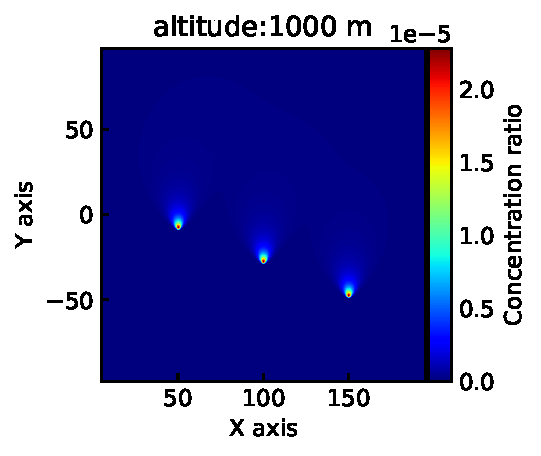
\includegraphics[width=\linewidth]{fig/sim_04_env_image1.pdf}
    \caption{強拡散大気条件}
    \label{fig:gas_map_high_diffuse}
  \end{subfigure}
  \hfill
  \begin{subfigure}{0.48\linewidth}
    \centering
    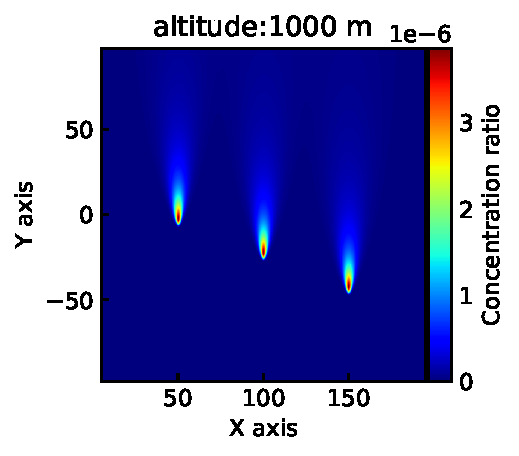
\includegraphics[width=\linewidth]{fig/sim_04_env_image2.pdf}
    \caption{弱拡散大気条件}
    \label{fig:gas_map_low_diffuse}
  \end{subfigure}
  \caption{大気拡散条件の違いによる地表面火山ガス分布}
  \label{fig:gas_map_compare}
\end{figure}

\begin{figure}
  \centering
  \begin{subfigure}{0.48\linewidth}
    \centering
    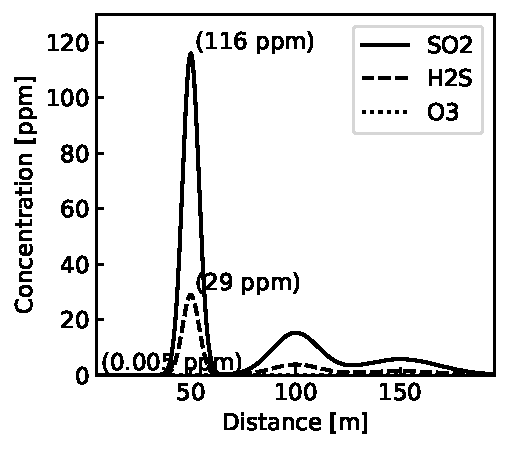
\includegraphics[width=\linewidth]{fig/sim_04_env1.pdf}
    \caption{強拡散大気条件}
    \label{fig:gas_setting_high_diffuse}
  \end{subfigure}
  \hfill
  \begin{subfigure}{0.48\linewidth}
    \centering
    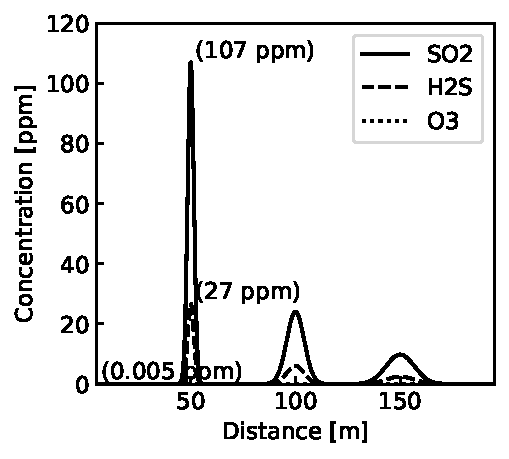
\includegraphics[width=\linewidth]{fig/sim_04_env2.pdf}
    \caption{弱拡散大気条件}
    \label{fig:gas_setting_low_diffuse}
  \end{subfigure}
  \caption{大気拡散条件の違いによるライダー視線上の濃度分布設定}
  \label{fig:gas_setting_diffuse_compare}
\end{figure}

\begin{figure}
  \centering
    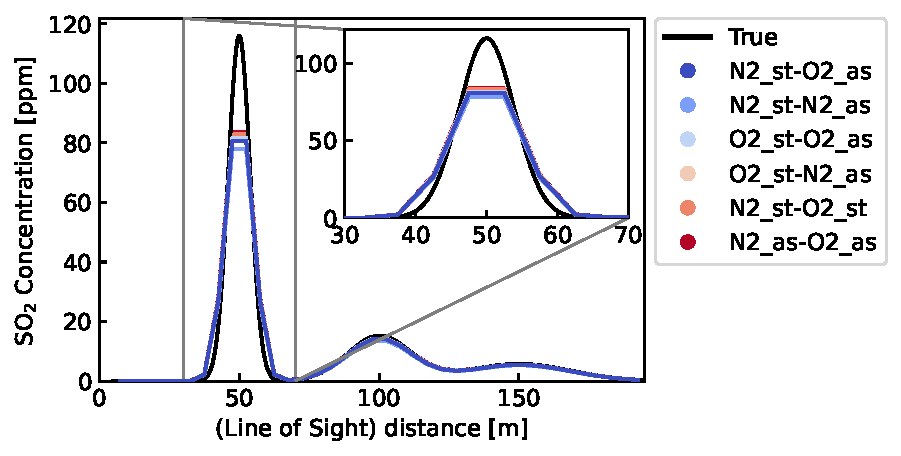
\includegraphics{fig/sim_04_plume_meas1.pdf}
    \caption{強拡散大気条件場における\ce{SO2}測定シミュレーション}
    \label{fig:plume_meas_high_diffuse}  
\end{figure}

\begin{figure}
  \centering
    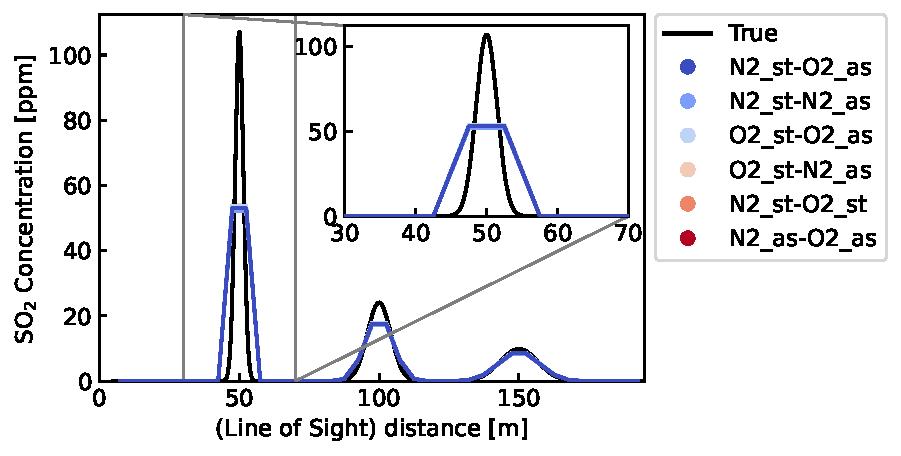
\includegraphics{fig/sim_04_plume_meas2.pdf}
    \caption{弱拡散大気条件場における\ce{SO2}測定シミュレーション}
    \label{fig:plume_meas_low_diffuse}  
\end{figure}
